\documentclass{article}\usepackage[]{graphicx}\usepackage[]{xcolor}
% maxwidth is the original width if it is less than linewidth
% otherwise use linewidth (to make sure the graphics do not exceed the margin)
\makeatletter
\def\maxwidth{ %
  \ifdim\Gin@nat@width>\linewidth
    \linewidth
  \else
    \Gin@nat@width
  \fi
}
\makeatother

\definecolor{fgcolor}{rgb}{0.345, 0.345, 0.345}
\newcommand{\hlnum}[1]{\textcolor[rgb]{0.686,0.059,0.569}{#1}}%
\newcommand{\hlsng}[1]{\textcolor[rgb]{0.192,0.494,0.8}{#1}}%
\newcommand{\hlcom}[1]{\textcolor[rgb]{0.678,0.584,0.686}{\textit{#1}}}%
\newcommand{\hlopt}[1]{\textcolor[rgb]{0,0,0}{#1}}%
\newcommand{\hldef}[1]{\textcolor[rgb]{0.345,0.345,0.345}{#1}}%
\newcommand{\hlkwa}[1]{\textcolor[rgb]{0.161,0.373,0.58}{\textbf{#1}}}%
\newcommand{\hlkwb}[1]{\textcolor[rgb]{0.69,0.353,0.396}{#1}}%
\newcommand{\hlkwc}[1]{\textcolor[rgb]{0.333,0.667,0.333}{#1}}%
\newcommand{\hlkwd}[1]{\textcolor[rgb]{0.737,0.353,0.396}{\textbf{#1}}}%
\let\hlipl\hlkwb

\usepackage{framed}
\makeatletter
\newenvironment{kframe}{%
 \def\at@end@of@kframe{}%
 \ifinner\ifhmode%
  \def\at@end@of@kframe{\end{minipage}}%
  \begin{minipage}{\columnwidth}%
 \fi\fi%
 \def\FrameCommand##1{\hskip\@totalleftmargin \hskip-\fboxsep
 \colorbox{shadecolor}{##1}\hskip-\fboxsep
     % There is no \\@totalrightmargin, so:
     \hskip-\linewidth \hskip-\@totalleftmargin \hskip\columnwidth}%
 \MakeFramed {\advance\hsize-\width
   \@totalleftmargin\z@ \linewidth\hsize
   \@setminipage}}%
 {\par\unskip\endMakeFramed%
 \at@end@of@kframe}
\makeatother

\definecolor{shadecolor}{rgb}{.97, .97, .97}
\definecolor{messagecolor}{rgb}{0, 0, 0}
\definecolor{warningcolor}{rgb}{1, 0, 1}
\definecolor{errorcolor}{rgb}{1, 0, 0}
\newenvironment{knitrout}{}{} % an empty environment to be redefined in TeX

\usepackage{alltt}
\usepackage{amsmath} %This allows me to use the align functionality.
                     %If you find yourself trying to replicate
                     %something you found online, ensure you're
                     %loading the necessary packages!
\usepackage{amsfonts}%Math font
\usepackage{graphicx}%For including graphics
\usepackage{hyperref}%For Hyperlinks
\usepackage[shortlabels]{enumitem}% For enumerated lists with labels specified
                                  % We had to run tlmgr_install("enumitem") in R
\hypersetup{colorlinks = true,citecolor=black} %set citations to have black (not green) color
\usepackage{natbib}        %For the bibliography
\setlength{\bibsep}{0pt plus 0.3ex}
\bibliographystyle{apalike}%For the bibliography
\usepackage[margin=0.50in]{geometry}
\usepackage{float}
\usepackage{multicol}

%fix for figures
\usepackage{caption}
\newenvironment{Figure}
  {\par\medskip\noindent\minipage{\linewidth}}
  {\endminipage\par\medskip}
\IfFileExists{upquote.sty}{\usepackage{upquote}}{}
\begin{document}

\vspace{-1in}
\title{Lab 10 -- MATH 240 -- Computational Statistics}

\author{
  Camilo Granada Cossio \\
  Colgate University  \\
  Department of Mathematics  \\
  {\tt cgranadacossio@colgate.edu}
}

\date{}

\maketitle

\begin{multicols}{2}
%\raggedcolumns % If your spacing gets messed up try uncommenting 
                % this line
\begin{abstract}

In this lab, we explored how sample size and population proportion affect the margin of error in survey sampling. We conducted simulation studies and apply the Wilson margin of error formula to compute and visualize margins of error. Our findings demonstrate that while larger sample sizes generally reduce margin of error, the true proportion play a crucial role, especially at the extremes. This analysis provide better context for interpreting polling results like those reported by Gallup.

\end{abstract}

\noindent \textbf{Keywords:} What topics does the lab cover concerning class? List 3-4 key terms here, separated by semicolons.

\section{Introduction}

Public opinion polls often report a fixed or rounded margin of error, such as  $\pm 4\%$, but this simplification hides important nuances. The margin of error depends not only on the sample size but also on the estimated proportion of success. In this lab, we investigate how both factors contribute to uncertainty in polling estimates.

We begin by using simulated polling data to visualize the sampling distribution of the sample proportion under assumed population parameters. Then, we use resampling techniques to examine variation. Finally, we compute margins of error using the Wilson margin of error formula across a range of values to generalize our findings.

\subsection{Intro Subsection}
Gallup states a single margin of error for their polls. However, the sampling distribution's spread varies depending on the true proportion being estimated. When the true proportion is close to $0$ or $1$, variability is constrained, and the margin of error is smaller. This lab aims to make that relationship clear through simulations and mathematical reasoning.

\section{Methods}

We conducted three main analyses:
\begin{enumerate}
\item Simulation study: We assumed a true proportion of $0.39$ and generated $10000$ samples for various sample sizes using \texttt{rbinom()}. We visualized the sampling distributions and calculated the middle $95\%$ range of simulated sample proportions.
\item Resampling: We simulated an original sample of $1004$ individuals with $39\%$ satisfaction and resampled $10000$ times with replacement to estimate sampling variability.
\item Wilson margin of error formula: We computed the margin of error using the Wilson formula across values of sample size ($100$ to $2000$) and true proportion ($0.01$ to $0.99$). This allowed us to create a heatmap of margin of error as a function of both variables using \texttt{geom\_raster()}.
\end{enumerate}

\texttt{R} packages used include \texttt{tidyverse} \citep{tidyverse} and \texttt{ggplot2} \citep{ggplot} for data manipulation and visualization.

\subsection{Mathematical Derivation}

We used the Wilson margin of error formula:

\[
\text{MOE}_{\text{Wilson}} = z_{1-\alpha/2} \times \frac{ \sqrt{ n\hat{p}(1-\hat{p}) + \frac{{z_{1-\alpha/2}}^2}{4} } }{ n + {z_{1-\alpha/2}}^2 }
\]


where $z_{1-\alpha/2}^2$ is the critical value from the standard normal distribution ($1.96$ for $95\%$ confidence).


\section{Results}

We began with a simulation assuming p = $0.39$ and n = $1000$, and found that the middle $95\%$ range of sample proportions was approximately [$0.361$, $0.419$], giving a margin of error of about $2.9\%$. When we doubled the sample size to $2000$, the margin of error shrank to about $2.1\%$, matching our theoretical expectations.

In the resampling section, we created a sample of $390$ satisfied and $610$ unsatisfied responses, and conducted $10000$ resamples. The histogram of sample proportions mirrored the previous simulation, reinforcing the expected behavior of sampling variability.

Using the Wilson margin of error formula, we computed the margin of error across a grid of n and p values. A \texttt{geom\_raster()} plot revealed that the margin of error is highest around p = $0.5$ and decreases toward the boundaries at $0$ and $1$. It also decreases as sample size increases, though with diminishing returns.

\section{Discussion}

Our simulations and mathematical calculations show that a fixed margin of error (like $\pm 4\%$) is overly simplistic. While larger samples do reduce variability, the proportion of interest strongly influences the precision of estimates. The Wilson margin of error provides a more nuanced and accurate measure of uncertainty, especially for small or extreme values of p.

For poll readers, this means interpreting results with caution. A statement like $39\%$ $\pm 4\%$ is only valid under specific assumptions, and real-world data may have more or less uncertainty.

Future polls should report margins of error as a function of both sample size and observed proportion, or at least clarify the assumptions behind a fixed error range.


%%%%%%%%%%%%%%%%%%%%%%%%%%%%%%%%%%%%%%%%%%%%%%%%%%%%%%%%%%%%%%%%%%%%%%%%%%%%%%%%
% Bibliography
%%%%%%%%%%%%%%%%%%%%%%%%%%%%%%%%%%%%%%%%%%%%%%%%%%%%%%%%%%%%%%%%%%%%%%%%%%%%%%%%
\vspace{2em}

\begin{tiny}
\bibliography{bib}
\end{tiny}
\end{multicols}

%%%%%%%%%%%%%%%%%%%%%%%%%%%%%%%%%%%%%%%%%%%%%%%%%%%%%%%%%%%%%%%%%%%%%%%%%%%%%%%%
% Appendix
%%%%%%%%%%%%%%%%%%%%%%%%%%%%%%%%%%%%%%%%%%%%%%%%%%%%%%%%%%%%%%%%%%%%%%%%%%%%%%%%
\newpage
\onecolumn
\section{Appendix}

\begin{figure}[h]
\centering
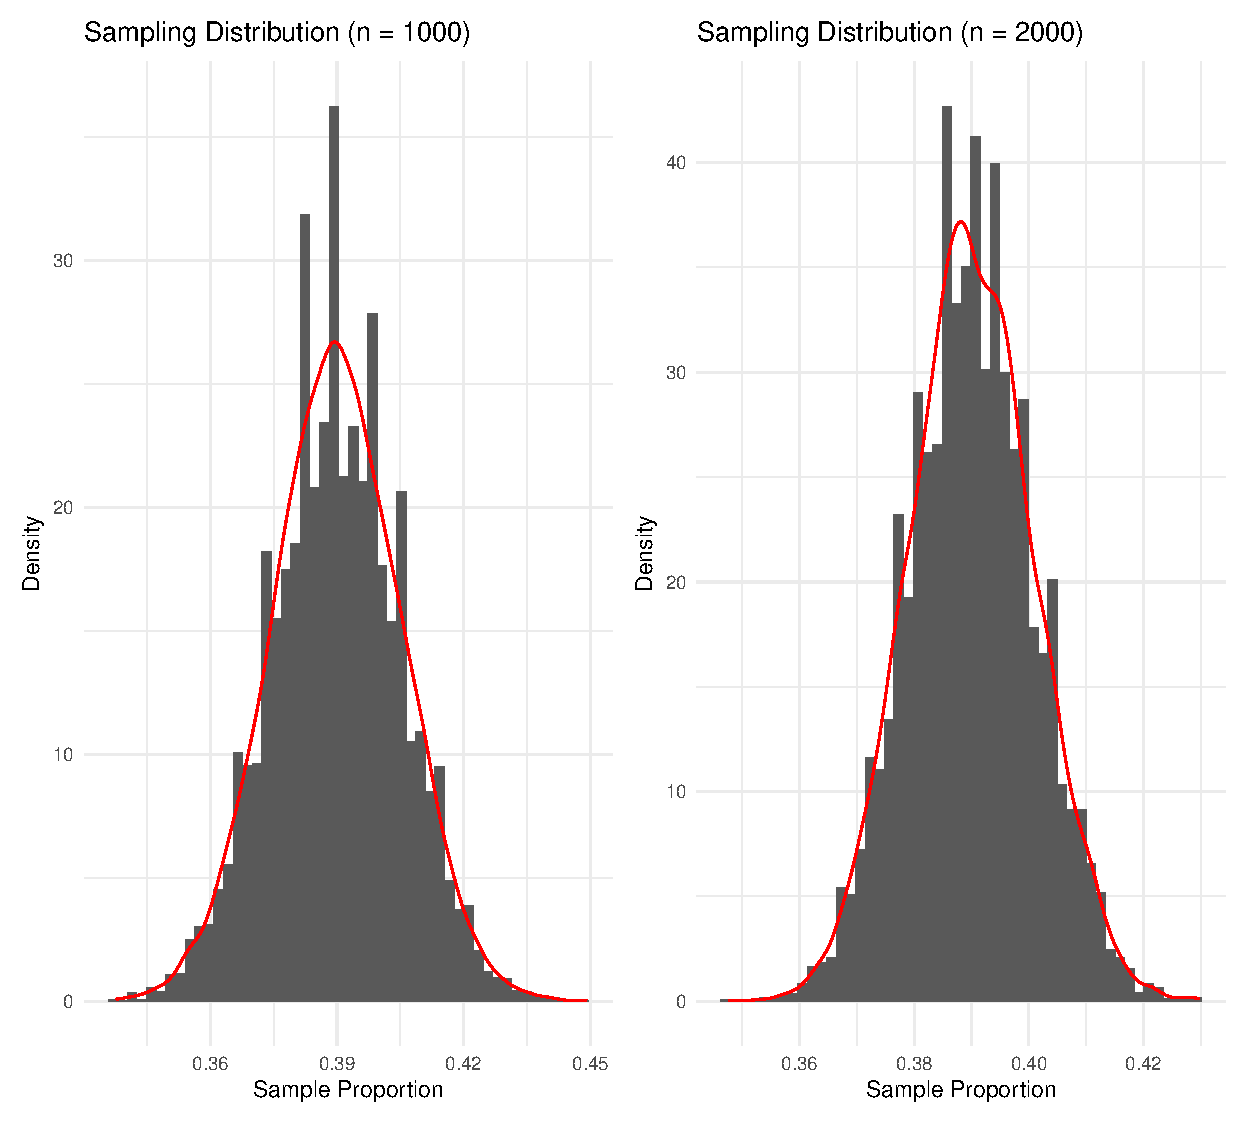
\includegraphics[width=0.9\textwidth]{Sampling_distributions.pdf}
\caption{Sampling Distributions for n = 1000 n = 2000}
\end{figure}

\begin{figure}[h]
\centering
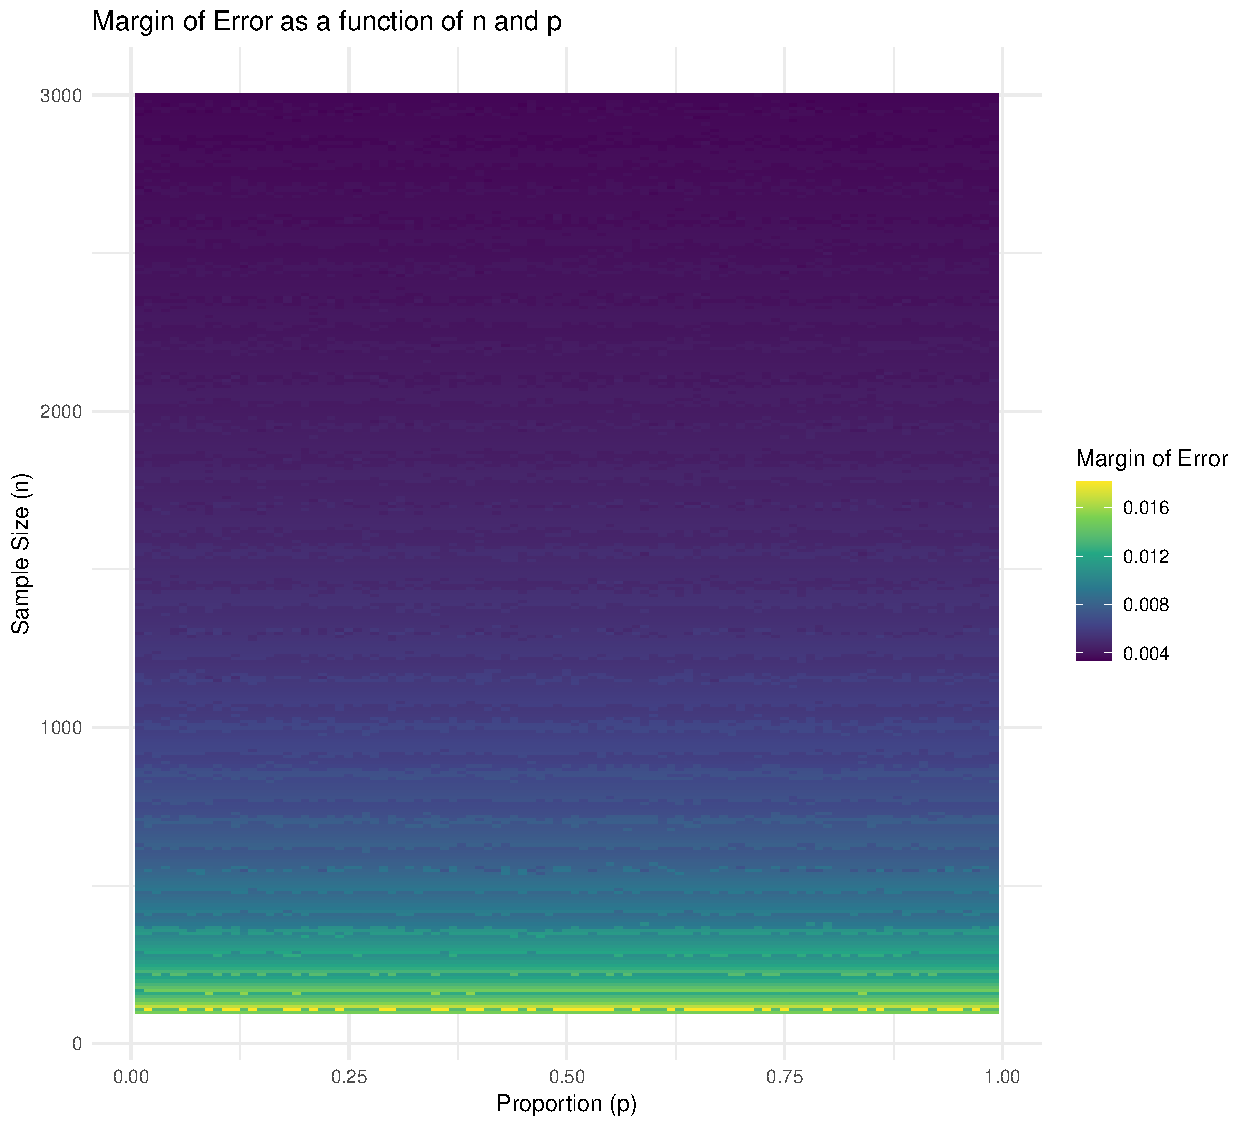
\includegraphics[width=0.9\textwidth]{MOEheatmap.pdf}
\caption{Margin of Error Heatmap for Resampling of Gallup Data}
\end{figure}

\begin{figure}[h]
\centering
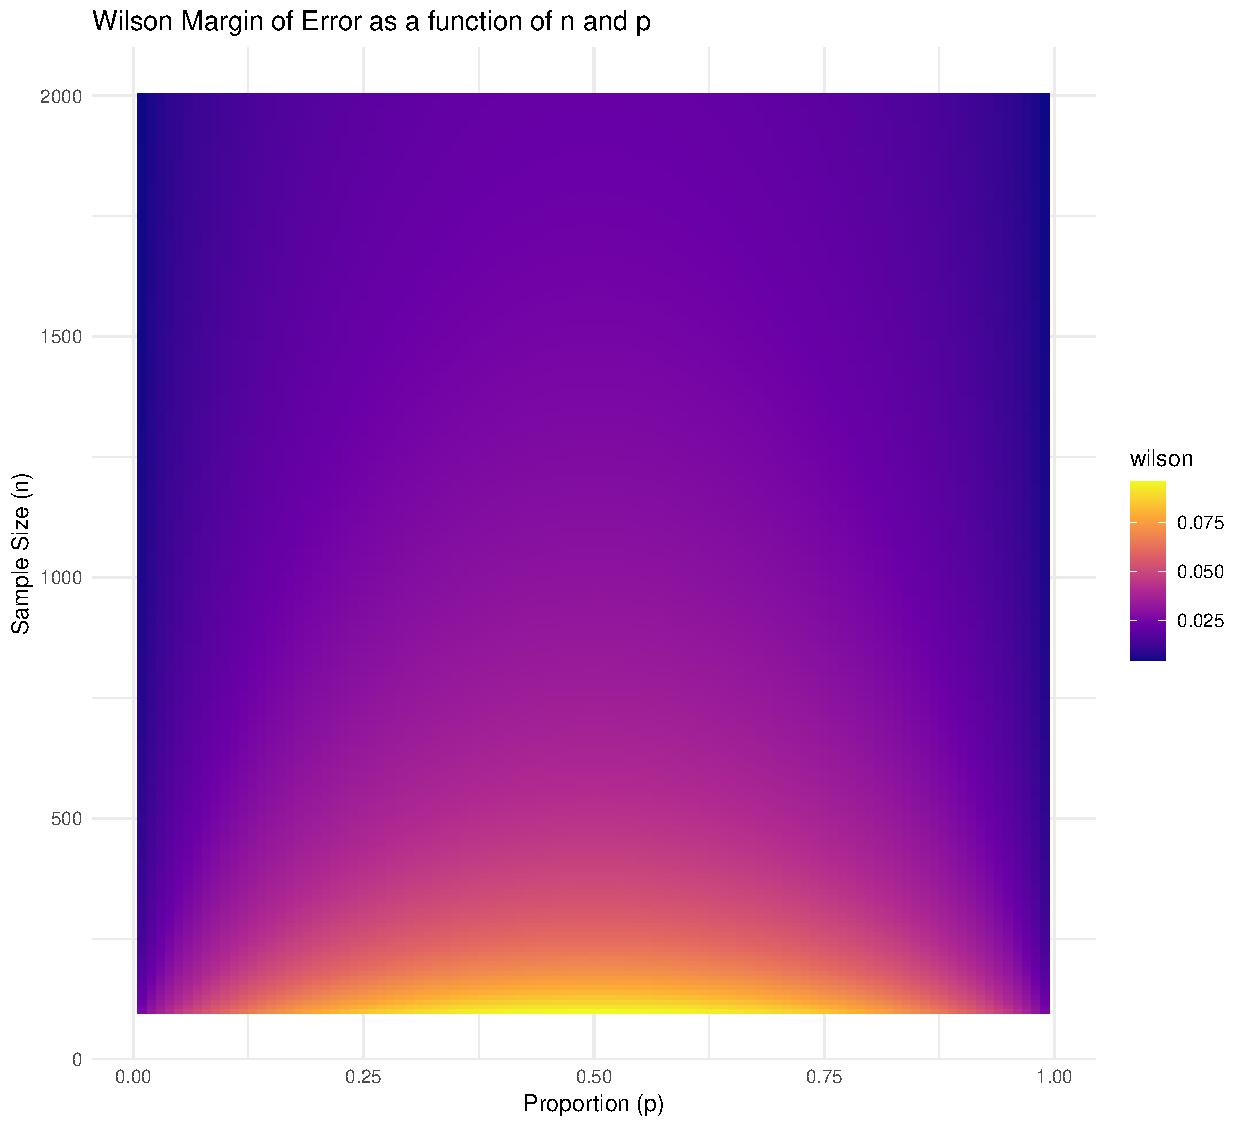
\includegraphics[width=0.9\textwidth]{Wilsonheatmap.pdf}
\caption{Wilson Margin of Error Formula Heatmap}
\end{figure}

\end{document}
